\chapter{Le logiciel Collec-Science}
\section{Historique}

L'unité de recherche \textit{Écosystèmes aquatiques et changements globaux} d'IRSTEA, à Cestas (33), récolte et manipule des échantillons prélevés sur le terrain (ou plutôt, principalement dans l'eau -- estuaires, lacs, rivières...), et les stocke, parfois pour des durées très longues : certaines campagnes de collecte ont eu lieu il y a plus de 40 ans.

De plus en plus, des échantillons anciens sont réanalysés (analyses génétiques, étude des ossements des oreilles ou otolithes...), au gré des questions scientifiques à traiter. 
Le besoin de recourir à un logiciel pour gérer ces matériels est devenu une priorité.

Dans un premier temps, quelques logiciels open-source susceptibles d'être utilisés ont été étudiés. Toutefois, leurs limites sont vite apparues : problème de pérennité, ancienneté du code, modèle de distribution parfois insatisfaisant (une licence open-source est obligatoire pour assurer la pérennité à longue échéance), résistance aux attaques informatiques, fonctionnalités insuffisantes ou inadaptées au besoin.

Dans un second temps, une étude des besoins réels a été menée. De nouvelles fonctionnalités ont été rajoutées, comme la gestion du stock de matériel utilisé sur le terrain, stocké dans un hangar.

L'unité de recherche s'intégrant au niveau régional avec d'autres organismes, des collaborations avec l'Observatoire Aquitain des Sciences de l'Univers (OASU) ou l'université de La Rochelle ont été envisagées.
Des échanges productifs ont ainsi pu être mis en place, entre autres sur la gestion de l'étiquetage et le scannage des codes-barres.

Le logiciel a largement évolué suite à ces échanges, de nombreuses fonctionnalités ont été rajoutées ou modifiées pour tenir compte des besoin des partenaires potentiels. 

Les délais de développement de la première version opérationnelle se sont étalés sur 9 mois, entre la définition des besoins et le développement proprement dit. 
La première version est parue à l'automne 2016, la version 2.0 est sortie en mai 2018.

Le code comprend environ 15800 lignes (commentaires compris), dont 7600 concernent l'affichage des pages web. Il a été écrit en PHP, les pages web sont générées en HTML et Javascript avec le composant Smarty.

\section{Fonctionnalités générales}

\begin{figure}[H]
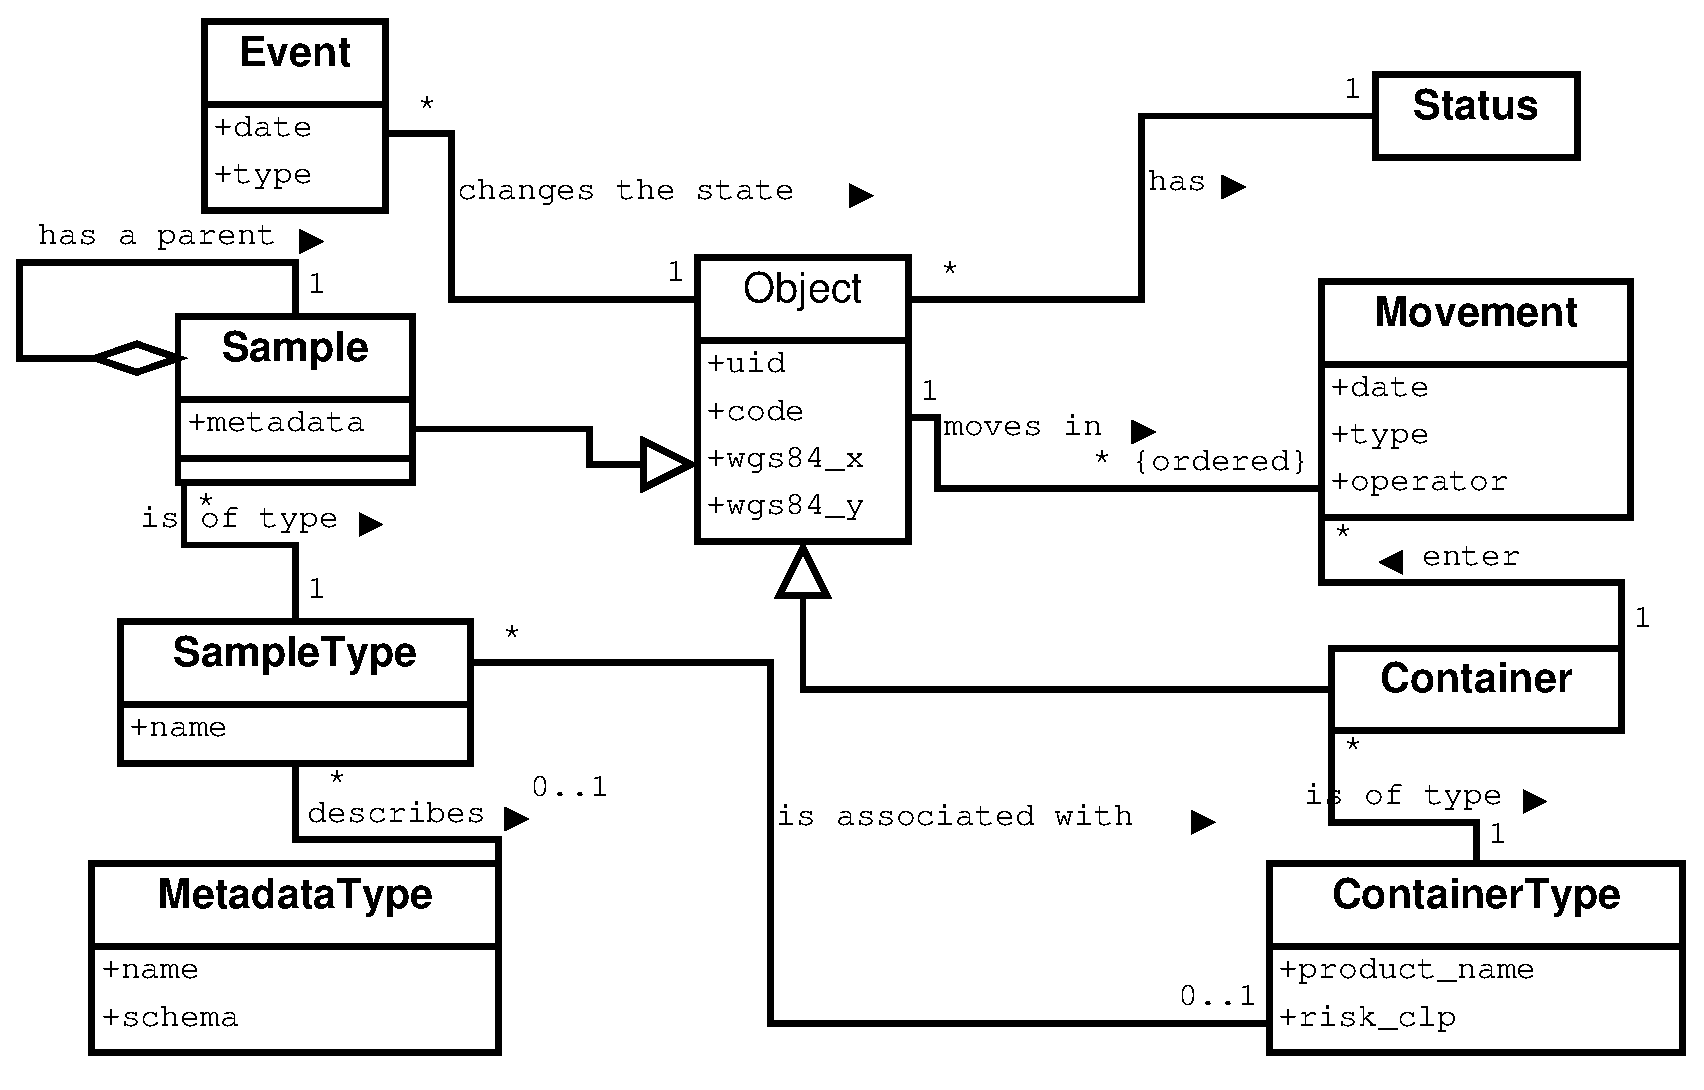
\includegraphics[width=\linewidth]{images/classes2}
\caption{Représentation objet de la base de données}
\end{figure}


Deux types d'objets sont manipulés dans l'application :
\begin{itemize}
\item des conteneurs (container), qui peuvent contenir des objets de tout type : d'autres conteneurs ou des échantillons. Ils peuvent être de différentes nature : site, bâtiment, salle, armoire, caisse, éprouvette... Les types de conteneurs décrivent également le produit de conservation utilisé et le risque associé (brûlure, cancérogène, etc.) ;
\item des échantillons (sample), qui peuvent être associés à un type de conteneur : il y a de nombreux cas où l'échantillon lui-même se confond avec son contenant, par exemple quand le résultat d'une pêche n'est pas trié et est stocké dans un bocal.
\end{itemize}

Un échantillon ou un conteneur sont issus d'un objet unique, qui est doté :
\begin{itemize}
\item d'un numéro unique, l'\textbf{UID}, qui sert de référence dans le logiciel ;
\item d'un identifiant métier, qui servira à le retrouver facilement (le logiciel permet également de définir d'autres identifiants).
\end{itemize}

Un objet peut subir un certain nombre d'événements, voire être réservé (fonctionnalité très simplifiée, seul le recouvrement de deux périodes de réservation est signalé).

Tout objet peut être étiqueté. Les étiquettes peuvent comprendre un code-barre 2D de type QRCode, qui pourra être lu soit à partir d'un terminal dédié (douchette), soit avec une tablette ou un smartphone, l'application disposant d'un module capable d'activer la caméra depuis le navigateur et de scanner le code-barre.

Un échantillon est obligatoirement rattaché à une collection. Seuls les les personnes rattachées à celle-ci peuvent modifier les informations le concernant. 

Pour mieux décrire les échantillons, il est possible de leur rattacher quelques informations \og métier \fg{}, appelées ici \textit{métadonnées}. Les types de métadonnées, totalement paramétrables, sont rattachés aux types d'échantillons.

Un échantillon peut être subdivisé en d'autres échantillons. Par exemple, des otolithes (os de l'oreille) peuvent être extraits d'un poisson. Le logiciel permet de créer un nouvel échantillon à partir d'un autre, qui peut être d'un autre type le cas échéant, et qui restera associé au parent. 

Enfin, dans certains cas de figures, un échantillon peut être composé de plusieurs éléments indifférenciés, par exemple plusieurs écailles de poisson prélevées et conservées ensemble. Le logiciel permet d'indiquer les prélèvements et les restitutions réalisées, et affiche le solde (théorique !) restant.

\section{Technologie employée}
\subsection{Base de données}

L'application a été conçue pour fonctionner avec Postgresql, en version 9.5. Les versions antérieures peuvent être utilisées, mais seule cette version dispose d'un type de données JSON qui permet de stocker les informations métiers.

\subsection{Langage de développement et framework utilisé}
Le logiciel a été écrit en PHP, en s'appuyant sur le framework \textit{Prototypephp} \cite{prototypephp}, développé parallèlement par l'auteur du logiciel.

Il utilise la classe \textit{Smarty} \cite{smarty} pour gérer l'affichage des pages HTML. Celles-ci sont générées en utilisant \textit{Jquery} \cite{jquery}  et divers composants associés. Le rendu général est réalisé avec \textit{Bootstrap} \cite{bootstrap}.

Les étiquettes sont générées en utilisant FOP \cite{fop}, une classe Java qui crée des fichiers PDF à partir d'un fichier XML contenant les données et un fichier de transformation au format XSL.

\subsection{Liste des composants externes utilisés}

\begin{longtable}{|>{\raggedright\arraybackslash}p{3cm}|c|c|>{\raggedright\arraybackslash}p{3cm}|>{\raggedright\arraybackslash}p{3cm}|}
\hline 
\textbf{Nom} & \textbf{Version} & \textbf{Licence} & \textbf{Usage} & \textbf{Site} \\ 
\hline 
\endhead
PrototypePHP & branche bootstrap & LGPL & Framework & \href{https://github.com/equinton/prototypephp}{github.com/ equinton/ prototypephp} \\ 
Smarty & 3.1.31 & LGPL & Générateur de pages HTML & \href{http://www.smarty.net}{www.smarty.net} \\ 
Smarty-gettext & 1.2.0 & LGPL & Support multi-langues pour Smarty & \\
PHPCAS & 1.3.5 & Apache 2.0 & Identification auprès d'un serveur CAS & \href{https://wiki.jasig.org/display/CASC/phpCAS}{wiki.jasig.org/ display/ CASC/ phpCAS} \\ 
PHPQRCODE &  1.1.4 & LGPL & Génération des qrcodes & \\
Zxcvbn-PHP & 0.3 & MIT & Vérification de la complexité des mots de passe & \\

\hline 
\caption{Table des composants PHP externes utilisés dans l'application}
\end{longtable} 

\begin{longtable}{|>{\raggedright\arraybackslash}p{3cm}|c|c|>{\raggedright\arraybackslash}p{3cm}|>{\raggedright\arraybackslash}p{3cm}|}
\hline 
\textbf{Nom} & \textbf{Version} & \textbf{Licence} & \textbf{Usage} & \textbf{Site} \\ 
\hline 
\endhead
Bootstrap & 3.0 & MIT & Présentation HTML & \href{http://getbootstrap.com}{get.bootstrap.com} \\ 
ComboBox & 1.0.1 & MIT & gestion des combobox & \\

JavaScript Cookie & 2.1.4 & MIT & Gestion des cookies dans le navigateur & \href{https://github.com/js-cookie/js-cookie}{github.com/ js-cookie/ js-cookie} \\ 

Datatables & 1.10.20 & MIT & Affichage des tableaux HTML & \href{http://www.datatables.net/}{www.datatables. net} \\ 

Datetime-moment &  & MIT & Formatage des dates dans les tableaux & \href{https://datatables.net/plug-ins/sorting/datetime-moment}{datatables.net/ plug-ins/ sorting/ datetime-moment} \\ 

Moment &  & MIT & Composant utilisé par datetime-moment & \href{http://momentjs.com} {momentjs.com}\\ 

JQuery & 3.3.1 & $\approx$ BSD & Commandes Javascript & \href{http://jquery.com/}{jquery.com} \\ 

JQuery-ui & 1.12.1 & $\approx$ BSD & Commandes Javascript pour les rendus graphiques & \href{http://jqueryui.com/}{jqueryui.com} \\ 

js.cookies & 0.0.4 & & Gestion des cookies & \\

leaflet & 1.3.4 & & Affichage des cartes OpenStreetMap & \\
leaflet-draw & 1.0.4 & & Dessin de polygones sur les cartes & \\
leaflet-mouse-position & 1.2.0 & & récupération de la position de la souris & \\
leaflet-marker-cluster & 1.4.1 & & & \\
leaflet-tylelayer-pouchdbcached & 1.0.0 & & Mise en cache de la cartographie & \\
pouchdb & 7.1.1 & & moteur de mise en cache & \\

Jquery-timepicker-addon &  & MIT & Time picker & \href{https://github.com/trentrichardson/jQuery-Timepicker-Addon}{github.com/ trentrichardson/ jQuery-Timepicker-Addon} \\ 

Magnific-popup & 1.1.0 & MIT & Affichage des photos & \href{http://dimsemenov.com/plugins/magnific-popup/}{dimsemenov .com/plugins/ magnific-popup/}\\ 

Smartmenus & 1.1.0 & MIT & Génération du menu HTML & \href{http://www.smartmenus .org}{www.smartmenus .org} \\ 
 
Openlayers & 4.2.0 & BSD & Affichage des cartes & \href{http://openlayers.org/}{openlayers.org} \\ 

qcode-decoder & & MIT & lecture de codes barres & \href{http://cirocosta.github.io/qcode-decoder/}{cirocosta.github .io/qcode-decoder}\\

Html5-qrcode &  & MIT & Lecture des QRcodes &  \href{https://github.com/dwa012/html5-qrcode}{github.com/ dwa012/ html5-qrcode} \\ 

AlpacaJS & 1.5.23 & Apache 2 & Génération et saisie des métadonnées & 
\href{http://www.alpacajs.org/}{www.alpacajs.org}\\

handlebars & 4.5.3 & & Gestion des boutons dans AlpacaJS & \\
zxcvbn & 4.4.2 & & Vérification de la complexité des mots de passe & \\
\hline
\caption{Table des composants Javascript externes utilisés dans l'application}
\end{longtable} 

\section{Sécurité}

L'application a été conçue pour résister aux attaques dites opportunistes selon la nomenclature ASVS v3 \cite{asvs} de l'OWASP \cite{owasp}. Des tests d'attaque ont été réalisés en août 2016 avec le logiciel ZapProxy \cite{zaproxy}, et n'ont pas détecté de faiblesse particulière.

La gestion des droits est conçue pour :
\begin{itemize}
\item qu'un utilisateur, membre d'une collection, ne puisse modifier que les échantillons qui y sont rattachés ;
\item que tout utilisateur disposant des droits de gestion peut procéder à une entrée ou une sortie d'un objet, quel qu'il soit ;
\item que les responsables d'une collection soient les seuls à pouvoir modifier les paramètres comme les types d'échantillons ou de conteneurs, les protocoles ou les opérations rattachées.
\end{itemize}
L'analyse de sécurité a mis en exergue un besoin de ne pas perdre d'information : si un échantillon est étiqueté et rangé, et que l'information est perdue, il y a de gros risques de ne plus pouvoir l'utiliser ultérieurement. Cela impose la mise en place d'un mécanisme de réplication de la base de données, à implémenter -- ou faire implémenter par des administrateurs du système -- directement dans Postgresql.

\section{Licence}
Le logiciel est diffusé selon les termes de la licence GNU AFFERO GENERAL PUBLIC LICENSE version 3, en date du 19 novembre 2007 \cite{agpl}.

\section{Copyright}

L'application a été déposée par IRSTEA auprès de l'Agence de protection des programmes \cite{app}, sous le numéro IDDN.FR.001.470013.000.S.C.2016.000.31500
